
\chapter{Introduction}

A disk contact graph is a graph for which there exists a mapping of all vertices to disks on the plane such that, if two vertices are connected, their respective disks are in contact with each other.
Since the formulation of the circle packing theorem~\cite{Koebe1936}, we know that every planar graph is a disk contact graph.

Various practical applications, such as wireless communication towers~\cite{Hale1980}, require us to consider the restricted case of \emph{unit disk graphs} (also known as \emph{coin graphs}), in which all disks in the graph's planar embedding are of one unit size.

Not every planar graph is a unit disk contact graph. Naturally, we have to consider the associated recognition problem: given a planar graph $G$, does it admit an embedding in the plane using unit disks? 
This problem is NP-hard~\cite{Breu1998}. The same complexity persists even restricting the problem only to trees, as shown by Bowen et al.~\cite{Bowen2015}.

\begin{figure}
    \centering
    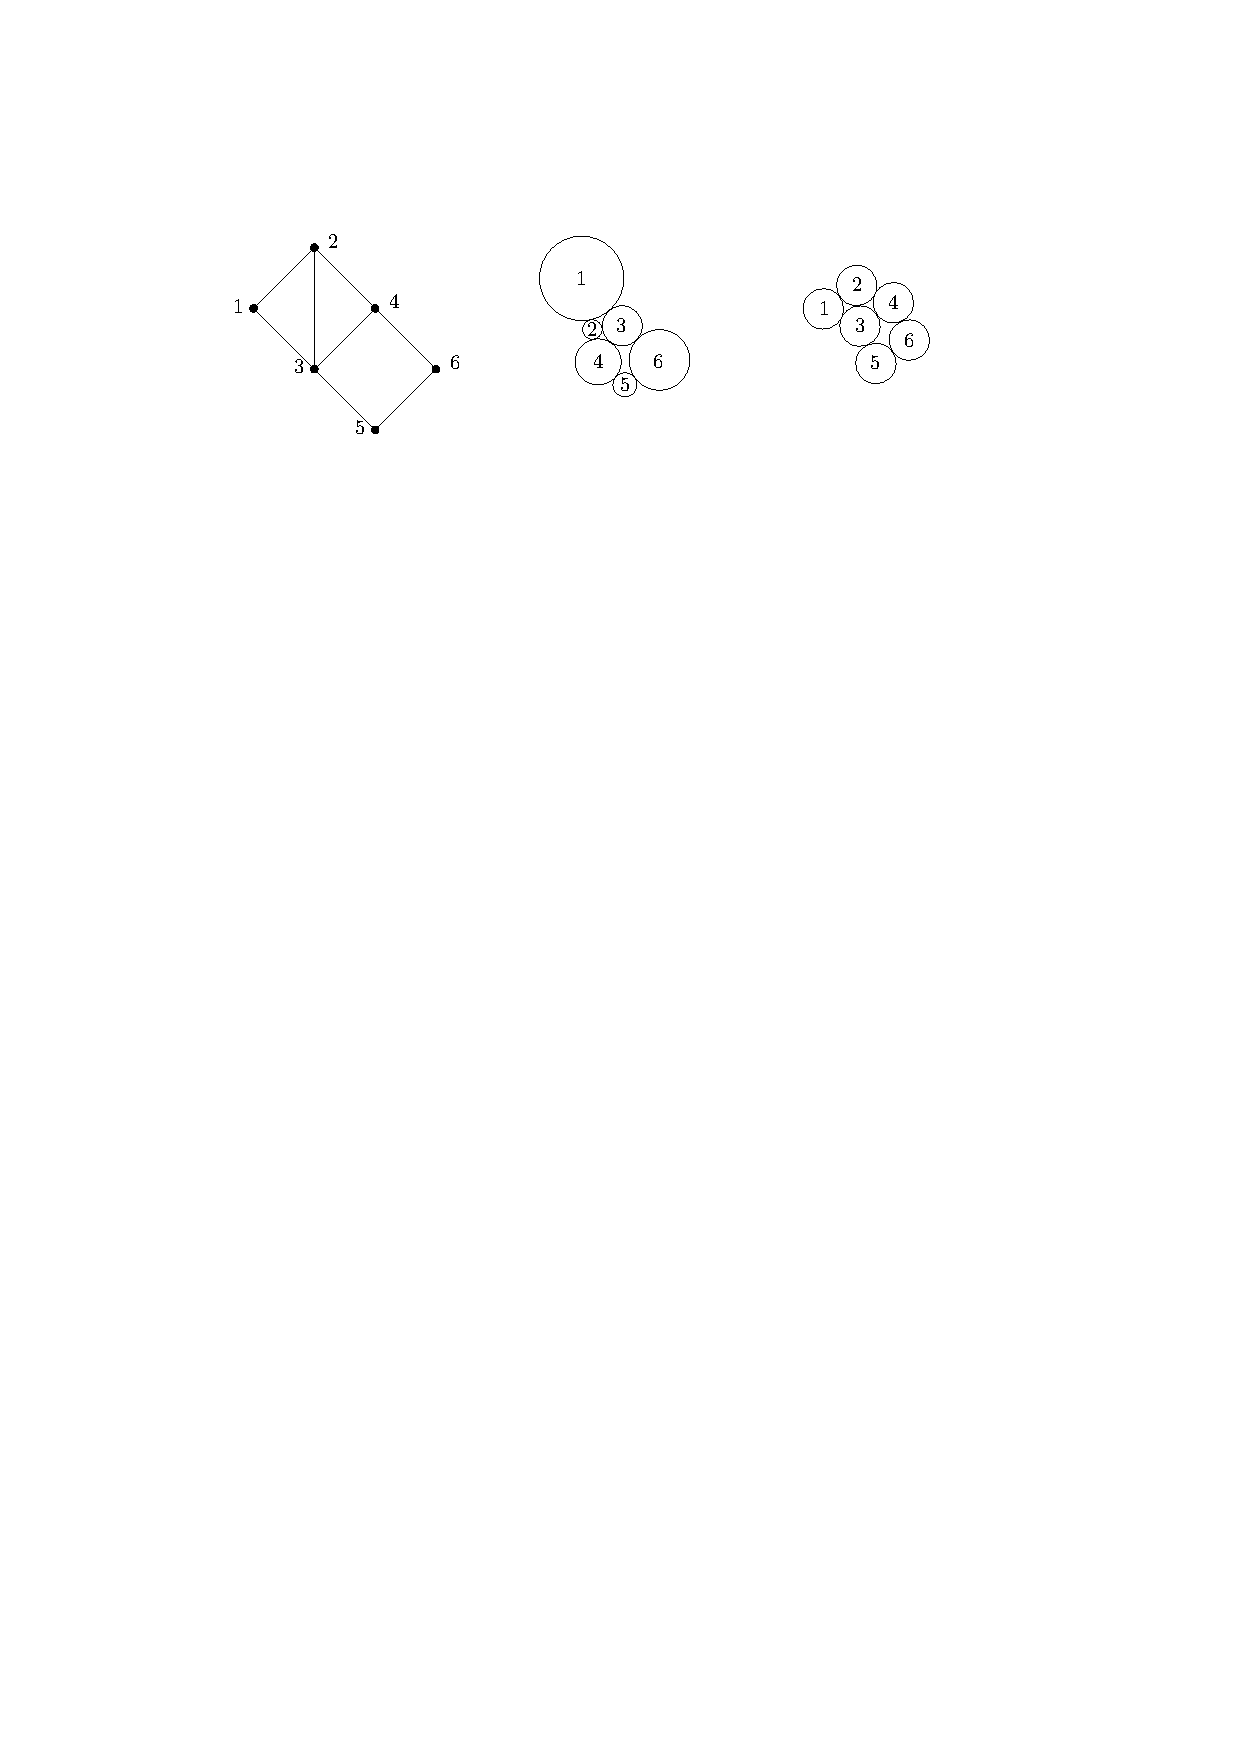
\includegraphics{graphics/ch1_introduction.pdf}
    \caption{Different representations of the same graph.}
    \label{fig:ch1_introduction}
\end{figure}

If even trees are too complex to decide in polynomial time, then where is the line of tractability? Coming at the problem from the other direction, we can identify graphs for which this problem is definitely in P.

A caterpillar is a tree which consists only of a string of connected vertices called a ``spine'' or ``backbone'', and an arbitrary number of leaf nodes connected to the spine.
It is possible to decide the problem for caterpillars in linear time~\cite{Klemz2015}~\cite{Cleve2020}. Klemz et al. show this result under the ``proper'' or ``strict'' mode of disk contact, where the interior-disjoint disks are in contact if and only if there is an edge between their nodes. Cleve uses the slightly modified notion of ``weak'' disk contact, in which the corresponding disks may touch even between unconnected vertices.

We conclude that the line between graph classes for which the recognition problem is tractable and those for which it remains intractable lies somewhere between caterpillars and trees. Perhaps there is some pertinent quality about them that determines the problem's complexity.

This thesis is concerned with the complexity of the recognition problem on the lobster, one such in-between class. Our approach uses the ``weak'' disk contact notion.

A lobster is a tree which, similar to the caterpillar, has a connected vertex string for a spine.
The spine vertices may further be connected to subtrees with a depth of at most two, i.e. ``expanding'' the caterpillar concept by one step from the leaves.

Our main question is whether the lobster, like the caterpillar, can be recognized in linear time. We also aim to provide a practical method of constructing a unit disk contact embedding for a given instance. Additionally, we are curious to know how fast and how accurate our solution is.

It is conjectured that lobsters are x-monotone, i.e. that any unit disk contact lobster can be embedded without any ``u-turns'' in the spine~\cite{Bhore2021}. With the \texttt{udcrgen} software developed in conjunction with this thesis, we provide a tool which can empirically evaluate such x-monotone lobsters through exhaustive enumeration and testing of small lobsters.

If lobsters are indeed x-monotone, and another assumption on the alignment of the embedding on a triangular grid also holds, it follows that the dynamic program implemented by \texttt{udcrgen} decides the problem in linear time~\cite{Bhore2021}. Beyond the asymptotic time constraints given by theory, our implementation should use prudent shortcuts and methods to achieve good performance in practice.

Furthermore, we present a heuristic to embed lobsters. Both approaches run in linear time, but the dynamic program requires us to consider an impractically large set of partial solutions. We examine both approaches with regards to correctness and run time.

The results thus presented narrow a gap in our understanding of the complexities of the unit disk contact problem. They offer tools for solving lobsters in particular, and a step towards further research.

In Chapter~2, we introduce all necessary terminology and formal definitions, building up to the embedding problems which we approach in the later chapters.
Chapter~3 delves into the literature which forms the basis of this work and other interesting related works.
Chapter~4 explains our reliable approach for deciding the UDCR problem for any given lobster in linear time. It covers theoretical and implementation aspects.
Chapter~5 explains our faster, but not always correct, approach to the same problem.
Chapter~6 describes our empirical evaluation of the two approaches. Using the implementation written in conjunction with this thesis, we exhaustively cover lobsters up to spine length 7. We compare our algorithms with regards to run time and correctness.
In Chapter~7, we summarize the results and consider open questions for future work.
